\documentclass[a4paper, 12pt]{article}		% general format

%%%% Charset
\usepackage{cmap}							% make PDF files searchable and copyable
\usepackage[utf8]{inputenc}					% accept different input encodings
\usepackage[T2A]{fontenc}					% russian font
\usepackage[russian]{babel}					% multilingual support (T2A)

%%%% Graphics
\usepackage[dvipsnames]{xcolor}			% driver-independent color extensions
\usepackage{graphicx}						% enhanced support for graphics
\usepackage{wrapfig}						% produces figures which text can flow around

%%%% Math
\usepackage{amsmath}						% American Mathematical Society (AMS) math facilities
\usepackage{amsfonts}						% fonts from the AMS
\usepackage{amssymb}						% additional math symbols

%%%% Typograpy (don't forget about cm-super)
\usepackage{microtype}						% subliminal refinements towards typographical perfection
\linespread{1.3}							% line spacing
\usepackage[left=2.5cm, right=1.5cm, top=2.5cm, bottom=2.5cm]{geometry}
\setlength{\parindent}{0pt}					% we don't want any paragraph indentation
\usepackage{parskip}
%\renewcommand{\chaptername}{}

%%%% Other
\usepackage{url}							% verbatim with URL-sensitive line breaks
%\DeclareUnicodeCharacter{00A0}{~}

%------------------------------------------------------------------------------
\usepackage{listings}						% typeset source code listings

% Цвета для кода
\definecolor{string}{HTML}{101AF9}			% цвет строк в коде
\definecolor{comment}{HTML}{3F7F5F}		% цвет комментариев в коде
\definecolor{keyword}{HTML}{5F1441}		% цвет ключевых слов в коде
\definecolor{morecomment}{HTML}{8000FF}	% цвет include и других элементов в коде
\definecolor{captiontext}{HTML}{FFFFFF}	% цвет текста заголовка в коде
\definecolor{captionbk}{HTML}{999999}		% цвет фона заголовка в коде
\definecolor{bk}{HTML}{FFFFFF}				% цвет фона в коде
\definecolor{frame}{HTML}{999999}			% цвет рамки в коде

% Настройки отображения кода
\lstset{
	language=C++,							% Язык кода по умолчанию
	morekeywords={*,...},					% если хотите добавить ключевые слова, то добавляйте
	% Цвета
	keywordstyle=\color{keyword}\ttfamily\bfseries,
	stringstyle=\color{string}\ttfamily,
	commentstyle=\color{comment}\ttfamily\itshape,
	morecomment=[l][\color{morecomment}]{\#},
	% Настройки отображения
	breaklines=true,						% Перенос длинных строк
	basicstyle=\ttfamily\footnotesize,		% Шрифт для отображения кода
	backgroundcolor=\color{bk},				% Цвет фона кода
	%frame=lrb,xleftmargin=\fboxsep,xrightmargin=-\fboxsep, % Рамка, подогнанная к заголовку
	frame=tblr								% draw a frame at all sides of the code block
	rulecolor=\color{frame},				% Цвет рамки
	tabsize=2,								% tab space width
	showstringspaces=false,					% don't mark spaces in strings
	% Настройка отображения номеров строк. Если не нужно, то удалите весь блок
	numbers=left,							% Слева отображаются номера строк
	stepnumber=1,							% Каждую строку нумеровать
	numbersep=5pt,							% Отступ от кода
	numberstyle=\small\color{black},		% Стиль написания номеров строк
	% Для отображения русского языка
	extendedchars=true,
	literate={Ö}{{\"O}}1
	 	{Ä}{{\"A}}1
	 	{Ü}{{\"U}}1
		{ß}{{\ss}}1
		{ü}{{\"u}}1
		{ä}{{\"a}}1
		{ö}{{\"o}}1
		{~}{{\textasciitilde}}1
		{а}{{\selectfont\char224}}1
		{б}{{\selectfont\char225}}1
		{в}{{\selectfont\char226}}1
		{г}{{\selectfont\char227}}1
		{д}{{\selectfont\char228}}1
		{е}{{\selectfont\char229}}1
		{ё}{{\"e}}1
		{ж}{{\selectfont\char230}}1
		{з}{{\selectfont\char231}}1
		{и}{{\selectfont\char232}}1
		{й}{{\selectfont\char233}}1
		{к}{{\selectfont\char234}}1
		{л}{{\selectfont\char235}}1
		{м}{{\selectfont\char236}}1
		{н}{{\selectfont\char237}}1
		{о}{{\selectfont\char238}}1
		{п}{{\selectfont\char239}}1
		{р}{{\selectfont\char240}}1
		{с}{{\selectfont\char241}}1
		{т}{{\selectfont\char242}}1
		{у}{{\selectfont\char243}}1
		{ф}{{\selectfont\char244}}1
		{х}{{\selectfont\char245}}1
		{ц}{{\selectfont\char246}}1
		{ч}{{\selectfont\char247}}1
		{ш}{{\selectfont\char248}}1
		{щ}{{\selectfont\char249}}1
		{ъ}{{\selectfont\char250}}1
		{ы}{{\selectfont\char251}}1
		{ь}{{\selectfont\char252}}1
		{э}{{\selectfont\char253}}1
		{ю}{{\selectfont\char254}}1
		{я}{{\selectfont\char255}}1
		{А}{{\selectfont\char192}}1
		{Б}{{\selectfont\char193}}1
		{В}{{\selectfont\char194}}1
		{Г}{{\selectfont\char195}}1
		{Д}{{\selectfont\char196}}1
		{Е}{{\selectfont\char197}}1
		{Ё}{{\"E}}1
		{Ж}{{\selectfont\char198}}1
		{З}{{\selectfont\char199}}1
		{И}{{\selectfont\char200}}1
		{Й}{{\selectfont\char201}}1
		{К}{{\selectfont\char202}}1
		{Л}{{\selectfont\char203}}1
		{М}{{\selectfont\char204}}1
		{Н}{{\selectfont\char205}}1
		{О}{{\selectfont\char206}}1
		{П}{{\selectfont\char207}}1
		{Р}{{\selectfont\char208}}1
		{С}{{\selectfont\char209}}1
		{Т}{{\selectfont\char210}}1
		{У}{{\selectfont\char211}}1
		{Ф}{{\selectfont\char212}}1
		{Х}{{\selectfont\char213}}1
		{Ц}{{\selectfont\char214}}1
		{Ч}{{\selectfont\char215}}1
		{Ш}{{\selectfont\char216}}1
		{Щ}{{\selectfont\char217}}1
		{Ъ}{{\selectfont\char218}}1
		{Ы}{{\selectfont\char219}}1
		{Ь}{{\selectfont\char220}}1
		{Э}{{\selectfont\char221}}1
		{Ю}{{\selectfont\char222}}1
		{Я}{{\selectfont\char223}}1
		{і}{{\selectfont\char105}}1
		{ї}{{\selectfont\char168}}1
		{є}{{\selectfont\char185}}1
		{ґ}{{\selectfont\char160}}1
		{І}{{\selectfont\char73}}1
		{Ї}{{\selectfont\char136}}1
		{Є}{{\selectfont\char153}}1
		{Ґ}{{\selectfont\char128}}1
}

% Для настройки заголовка кода
\usepackage{caption}
\DeclareCaptionFont{white}{\color{сaptiontext}}
\DeclareCaptionFormat{listing}{\parbox{\linewidth}{\colorbox{сaptionbk}{\parbox{\linewidth}{#1#2#3}}\vskip-4pt}}
%\captionsetup[lstlisting]{format=listing,labelfont=white,textfont=white}
\renewcommand{\lstlistingname}{Листинг} % Переименование Listings в нужное именование структуры

%------------------------------------------------------------------------------
\begin{document}

\begin{titlepage}
\thispagestyle{empty}

\begin{center}
Санкт-Петербургский государственный политехнический университет \\
Институт Информационных Технологий и Управления \\*
Кафедра компьютерных систем и программных технологий \\*
\hrulefill
\end{center}

\vspace{18em}

\begin{center}
\Large Отчёт по расчётной работе № 3 \\ по предмету «Системное программное обеспечение» \\
\end{center}

\vspace{1em}

% \linebreak
\begin{center}
\textsc{\textbf{Примитивы синхронизации в ОС Windows}}
\end{center}

\vspace{16em}

\begin{flushleft}
Работу выполнил студент гр. 53501/3\hrulefill Мартынов С. А. \\
\vspace{1.5em}
Работу принял преподаватель \hrulefill Душутина Е. В. \\
\end{flushleft}

\vspace{\fill}

\begin{center}
Санкт-Петербург \\
2014
\end{center}

\end{titlepage}
%------------------------------------------------
\setcounter{page}{2}
\tableofcontents
%------------------------------------------------
\newpage
\section*{Постановка задачи}
\addcontentsline{toc}{section}{Постановка задачи}

В рамках данной работы необходимо ознакомиться с основными примитивами синхронизации в ОС Windows, и выполнить практические задачи.
\vspace{2em}

Потоки разделяют целочисленный массив, в который заносятся производимые и извлекаются потребляемые данные. Для наглядности и контроля за происходящим в буфер помещается наращиваемое значение, однозначно идентифицирующее производителя и номер его очередной посылки.
\vspace{1em}

Код должен удовлетворять трем требованиям:
\begin{itemize}
\item потребитель не должен пытаться извлечь значение из буфера, если буфер пуст;
\item производитель не должен пытаться поместить значение в буфер, если буфер полон;
\item состояние буфера должно описываться общими переменными (индексами, счётчиками, указателями связанных списков и т.д.).
\end{itemize}
\vspace{1em}

Задание необходимо выполнить различными способами, применив следующие средства синхронизации доступа к разделяемому ресурсу:
\begin{itemize}
\item Мьютексы;
\item Семафоры;
\item Критические секции;
\item Объекты события;
\item Условные переменные;
\item Функции ожидания.
\end{itemize}

Создать аналогичные программы для множества потоков, количество которых можно задать из командной строки.

Программы должны предоставлять возможность завершения по таймеру либо по команде оператора.
\vspace{3em}

Отчёт должен содержать:
\begin{enumerate}
\item Результаты выполнения предложенных в методическом пособии программ и их анализ.
\item Решение задачи читатели-писатели таким образом, чтобы читатели не имели доступа к памяти по записи.
\item Более рациональное решение задачи читатели-писатель, используя другие средства синхронизации или их сочетание.
\item Клиент-серверное приложение для полной задачи читатели-писатели.
\item Программу читатели-писатели для сетевого функционирования (для этого необходимо выбрать подходящие средства IPC и синхронизации).
\item Решение задачи производители-потребители (разница с предыдущей задачей в возможности модификации считываемых данных).
\item Задачу "обедающие философы" с обоснованием выбранных средств синхронизации.
\end{enumerate}

\newpage
%------------------------------------------------
\section*{Введение}
\addcontentsline{toc}{section}{Введение}

В Windows реализована вытесняющая многозадачность - это значит, что в любой момент система может прервать выполнение одной нити и передать управление другой. Все нити, принадлежащие одному процессу, разделяют некоторые общие ресурсы - такие, как адресное пространство оперативной памяти или открытые файлы. Эти ресурсы принадлежат всему процессу, а значит, и каждой его нити. Следовательно, каждая нить может работать с этими ресурсами без каких-либо ограничений. Отсутствие ограничений приводит к известным проблемам, таким как гонка, тупик или голодание.

Именно поэтому необходим механизм, позволяющий потокам согласовывать свою работу с общими ресурсами. Этот механизм получил название механизма синхронизации нитей (thread synchronization).

Этот механизм представляет собой набор объектов операционной системы, которые создаются и управляются программно, являются общими для всех нитей в системе (некоторые - для нитей, принадлежащих одному процессу) и используются для координирования доступа к ресурсам. В качестве ресурсов может выступать все, что может быть общим для двух и более нитей - начиная с совместно используемого байта в оперативной памяти, и заканчивая чем-то совсем высокоуровневым, вроде записи в базе данных.

Объектов синхронизации существует несколько, основные это взаимоисключение (mutex), критическая секция (critical section), событие (event) и семафор (semaphore). Каждый из этих объектов реализует свой способ синхронизации. Любой объект синхронизации может находиться в так называемом сигнальном состоянии. Для каждого типа объектов это состояние имеет различный смысл. Нити могут проверять текущее состояние объекта и/или ждать изменения этого состояния и таким образом согласовывать свои действия. При этом гарантируется, что когда нить работает с объектами синхронизации (создаёт их, изменяет состояние) система не прервёт ее выполнения, пока она не завершит это действие. 

В данной работе рассмотрены основные механизмы на примере конкретных популярных задач. Часть кода приведена в листингах, но более подробная версия доступна по адресу \\ \url{https://github.com/SemenMartynov/SPbPU_SystemProgramming}.

\newpage
%------------------------------------------------
\section{Примитивы синхронизации}

Код задач в данном разделе разбит на файлы. Некоторые файлы (такие как система логирования) в разных проектах содержат одинаковый код. Для простоты восприятия информации, они вынесены в этот раздел (полную версию исходных кодов можно получит по ссылке на гитхаб, приведённой во введении).

В листинге 1 представлена реализация класса, который занимается логированием событий программы. Логирование может быть тихим (когда информация попадает в файл) или громким (когда информация записывается в файл и выводится на экран). При создании класса в качестве параметра передаётся номер процесса, это позволяет отличать логи разных потоков. Каждое событие сопровождается мекой времени.

\lstinputlisting[language=C++, caption={Реализация класса логера}]
{../../SynchronizationPrimitives/Mutex/Logger.cpp}

Сервисные функции представлены в листинге 2. Они используются для создания потоков и чтения конфигурационного файла.Если конфигурационный файл прочитать не удалось, используются значения по умолчанию. Сам конфигурационный файл может выглядеть следующим образом:
\begin{verbatim}
NumOfReaders= 10
ReadersDelay= 100
NumOfWriters= 10
WritersDelay= 200
SizeOfQueue= 10
ttl= 3
\end{verbatim}

\lstinputlisting[language=C++, caption={Сервисные функции}]
{../../SynchronizationPrimitives/Mutex/utils.cpp}

\newpage
%------------------------------------------------
\subsection{Использование мьютексов}

Объекты ядра «мьютексы» гарантируют потокам взаимоисключающий доступ к единственному ресурсу. Это отражено в название этих объектов (mutual exclusion, mutex). Они содержат счётчик числа пользователей, счетчик рекурсии и переменную, в которой запоминается идентификатор потока. Мьютексы ведут себя точно так же, как и критические секции. Однако, если последние являются объектами пользователь ского режима, то мьютексы — объектами ядра. Кроме того, единственный объектмью текс позволяет синхронизировать доступ к ресурсу нескольких потоков из разных процессов; при этом можно задать максимальное время ожидания доступа к ресурсу.

Идентификатор потока определяет, какой поток захватил мьютекс, а счетчик рекурсий - количество. У мьютексов много применений, и это наиболее часто используемые объекты ядра. Как правило, с их помощью защищают блок памяти, к которому обращается множество потоков Если бы потоки одновременно использовали какой-то блок памяти, данные в нем были бы повреждены. Мьютексы гарантируют, что любой поток получает монопольный доступ к блоку памяти, и тем самым обеспечивают целостность данных.

Листинг 3 демонстрирует инициализацию и закрытие мьютекса, который активно используется читателями (листинг 4) и писателями (листинг 5). Важно отметить, что этот мьютекс имеет пустое имя, следовательно не может использоваться сторонним процессом и служить средством IPC.

\lstinputlisting[language=C++, caption={Основной файл, демонстрирующий работу с мьютексами}]
{../../SynchronizationPrimitives/Mutex/main.cpp}

\lstinputlisting[language=C++, caption={Потоки читатели, синхронизация через мьютекс}]
{../../SynchronizationPrimitives/Mutex/threadReader.cpp}

\lstinputlisting[language=C++, caption={Потоки писатели, синхронизация через мьютекс}]
{../../SynchronizationPrimitives/Mutex/threadWriter.cpp}

На рисунке 1 показана работа потоков с мьютексом.

\begin{figure}[h!]
\centering
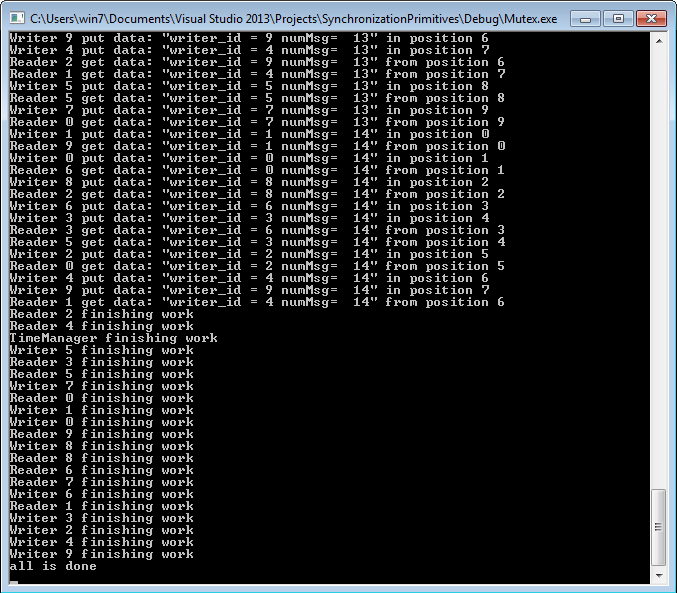
\includegraphics[scale=1]{res/001}
\caption{Использование мьютексов.}
\end{figure}

Файл с логом работы программы содержит почти аналогичный результат (различия в метках времени при переходе из состояния ожидания в состояние владения и обратно). Рисунок 2 показывает множество потоков, каждый из которых пишет свой файл с логом.

\begin{figure}[h!]
\centering
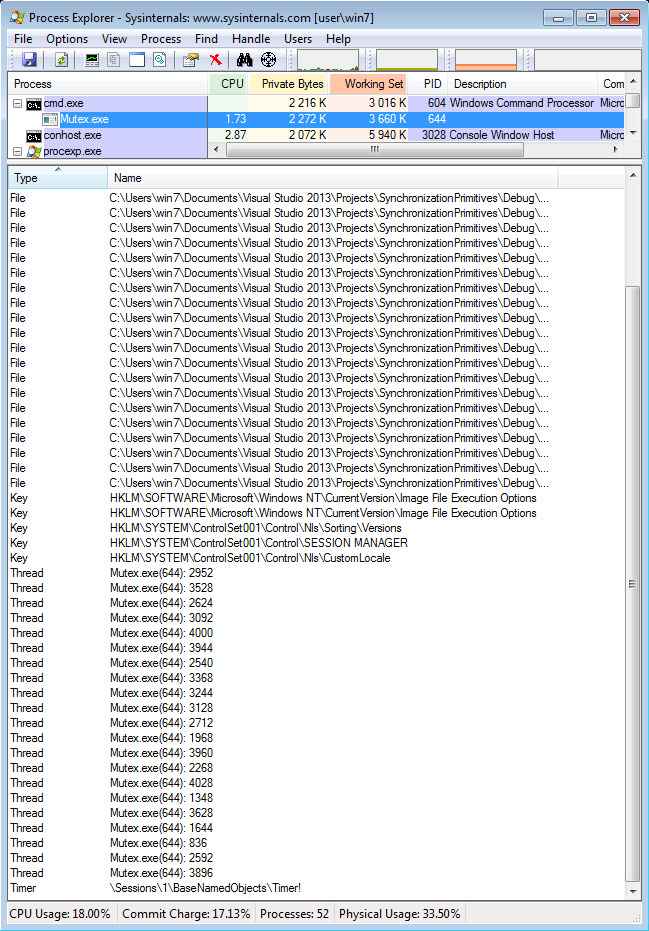
\includegraphics[scale=0.65]{res/pe_01}
\caption{Потоки и файлы с логами.}
\end{figure}


\newpage
%------------------------------------------------
\subsection{Использование семафоров}

Объекты ядра «семафор» используются для учета ресурсов Как и все объекты ядра, они содержат счетчик числа пользователей, но, кроме того, поддерживают два 32 битных значения со знаком: одно определяет максимальное число ресурсов (контролируемое семафором), другое используется как счетчик текущего числа ресурсов. Таким образом, семафор используются для учёта ресурсов и служат для ограничения одновременного доступа к ресурсу нескольких потоков. Используя семафор, можно организовать работу программы таким образом, что к ресурсу одновременно смогут получить доступ несколько потоков, однако количество этих потоков будет ограничено. Создавая семафор, указывается максимальное количество потоков, которые одновременно смогут работать с ресурсом. Каждый раз, когда программа обращается к семафору, значение счётчика ресурсов семафора уменьшается на единицу. Когда значение счётчика ресурсов становится равным нулю, семафор недоступен.

Как и в прошлом случае, Листинг 6 содержит основной файл, в котором семафор инициализируется, а используется он писателем и читателем в листингах 7 и 8.

\lstinputlisting[language=C++, caption={Основной файл, инициализация семафора со счётчиком 1}]
{../../SynchronizationPrimitives/Semaphore/main.cpp}
\newpage

\lstinputlisting[language=C++, caption={Потоки писатели, синхронизация через семафор}]
{../../SynchronizationPrimitives/Semaphore/threadWriter.cpp}

\lstinputlisting[language=C++, caption={Потоки читатели, синхронизация через семафор}]
{../../SynchronizationPrimitives/Semaphore/threadReader.cpp}

Результат работы на рисунке 3.

\begin{figure}[h!]
\centering
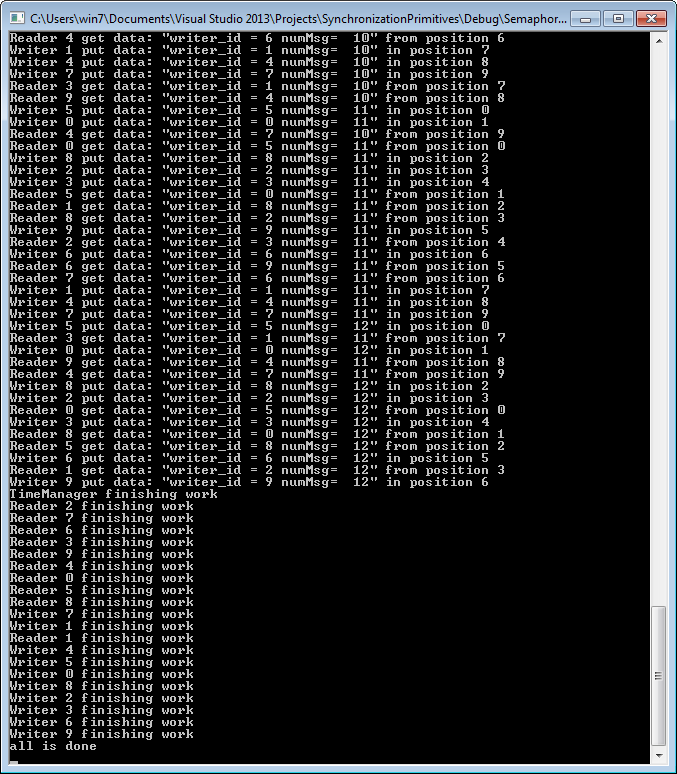
\includegraphics[scale=0.99]{res/002}
\caption{Использование семафоров.}
\end{figure}

Результат работы можно изучать и по логам программы. Листинг 9 содержит общий лог работы программы, листинг 10 показывает работу одного из писателей, а листинг 11 - одного из читателей.

\lstinputlisting[language={},caption={Общий протокол работы программы}]{res/Semaphore.log}
\newpage

\lstinputlisting[language={},caption={Протокол работы писателя}]{res/Semaphore.ThreadWriter.1.log}

\lstinputlisting[language={},caption={Протокол работы читателя}]{res/Semaphore.ThreadReader.1.log}

\newpage
%------------------------------------------------
\subsection{Критические секции}

Критическая секция (critical section) — это небольшой участок кода, который должен использоваться только одним потоком одновременно. Если в одно время несколько потоков попытаются получить доступ к критическому участку, то контроль над ним будет предоставлен только одному из потоков, а все остальные будут переведены в состояние ожидания до тех пор, пока участок не освободится.

Критический раздел анализирует значение специальной переменной процесса, которая используется как флаг, предотвращающий исполнение участка кода несколькими потоками одновременно.

Среди синхронизирующих объектов критические разделы наиболее просты. Инициализация критической секции показана в листинге 12 (при этом имя мекции ни где не указывается), а захват в листинге 13 и листинге 14 (для захвата нет ожидания события, секция оказывается захваченой когда это возможно).

\lstinputlisting[language=C++, caption={Основной файл, инициализирующий критическую секцию}]
{../../SynchronizationPrimitives/CriticalSection/main.cpp}

\lstinputlisting[language=C++, caption={Потоки писатели, синхронизация через семафор критическую секцию}]
{../../SynchronizationPrimitives/CriticalSection/threadWriter.cpp}

\newpage
\lstinputlisting[language=C++, caption={Потоки читатели, синхронизация через семафор критическую секцию}]
{../../SynchronizationPrimitives/CriticalSection/threadReader.cpp}

Демонстрация работы синхронизации через критическую секцию показана на рисунке 4.

\begin{figure}[h!]
\centering
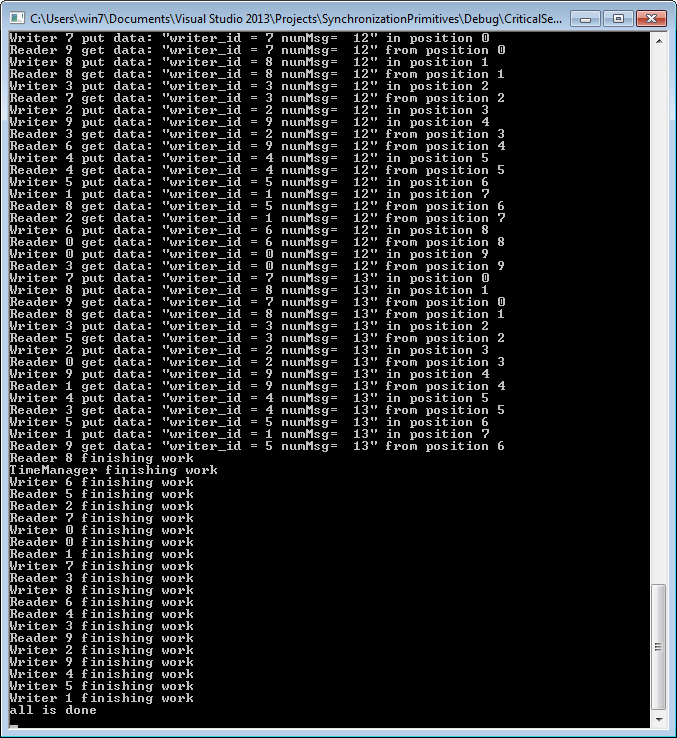
\includegraphics[scale=1]{res/003}
\caption{работа с критической секцией}
\end{figure}

\newpage
%------------------------------------------------
\subsection{Объекты-события в качестве средства синхронизации}

События обычно просто оповещают об окончании какой-либо операции, они также являются объектами ядра. Можно не просто явным образом освободить, но так же есть операция установки события. События могут быть ручным (manual) и единичными (single).

Единичное событие (single event) – это скорее общий флаг. Событие находится в сигнальном состоянии, если его установил какой-нибудь поток. Если для работы программы требуется, чтобы в случае возникновения события на него реагировал только один из потоков, в то время как все остальные потоки продолжали ждать, то используют единичное событие.

Ручное событие (manual event) — это не просто общий флаг для нескольких потоков. Оно выполняет несколько более сложные функции. Любой поток может установить это событие или сбросить (очистить) его. Если событие установлено, оно останется в этом состоянии сколь угодно долгое время, вне зависимости от того, сколько потоков ожидают установки этого события. Когда все потоки, ожидающие этого события, получат сообщение о том, что событие произошло, оно автоматически сбросится.

В листинге 15 просиходит инициализация и закрытие объектов-событий, а в листинге 16 и 17 происходит ожидание и захват.

\lstinputlisting[language=C++, caption={Основной файл инициализации объектов-событий}]
{../../SynchronizationPrimitives/Event/main.cpp}

\lstinputlisting[language=C++, caption={Потоки писатели, синхронизация через объекты-события}]
{../../SynchronizationPrimitives/Event/threadWriter.cpp}

\lstinputlisting[language=C++, caption={Потоки читатели, синхронизация через объекты-события}]
{../../SynchronizationPrimitives/Event/threadReader.cpp}

Рисунок 5 содержит результат работы, дублирующий лог программы.

\begin{figure}[h!]
\centering
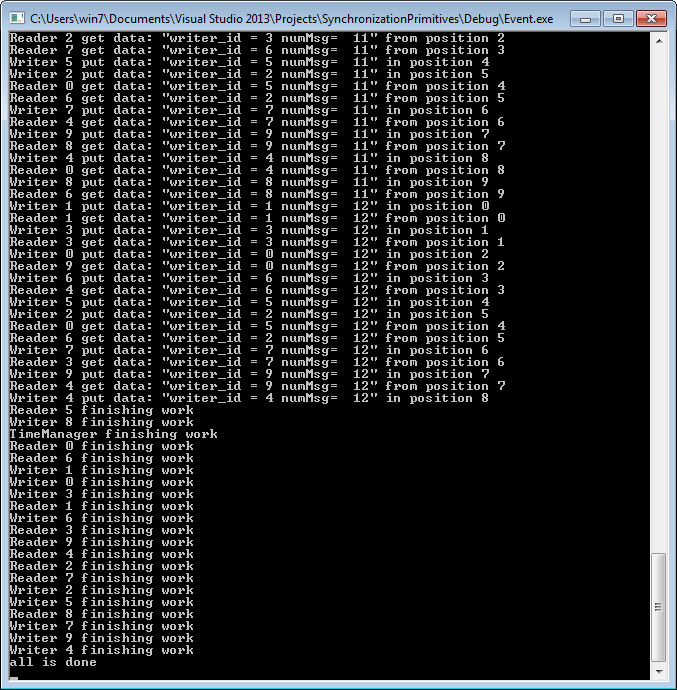
\includegraphics[scale=1]{res/004}
\caption{Объекты-события в качестве средства синхронизации.}
\end{figure}

\newpage
%------------------------------------------------
\subsection{Условные переменные}

Условные переменные- это объекты, поддерживающие операции ожидания и уведомления. Ожидание возможно только внутри какой-либо критической секции, то есть данная операция связана не только с какой-либо условной переменной, но еще и с соответствующим мьютексом. При этом возможны ситуации, когда, например, разные условные переменные должны быть связаны с одним и тем же мьютексом, в случае, если они относятся к одному и тому же ресурсу, но означают разные условия. Операция ожидания атомарно освобождает мьютекс и блокирует процесс до момента уведомления о том, что условие выполнено.

В листинге 18 происходит инициализация условных перемсенных, но для организации полноценной работы их не достаточно. Поэтому в качестве вспомогательного объекта синхронизации используется критическая секция.

\lstinputlisting[language=C++, caption={Основной файл инициализации примитивов синхронизации}]
{../../SynchronizationPrimitives/ConditionVariable/main.cpp}

Читатели (листинг 19) и писатели (листинг 20) входят в критическую секцию, но для работы ожидают условную переменную.

\lstinputlisting[language=C++, caption={Потоки читатели, синхронизация через условные переменные и критические секции}]
{../../SynchronizationPrimitives/ConditionVariable/threadReader.cpp}

\lstinputlisting[language=C++, caption={Потоки писатели, синхронизация через условные переменные и критические секции}]
{../../SynchronizationPrimitives/ConditionVariable/threadWriter.cpp}
\newpage

Результат работы сразу с двумя примитивами показан на рисунке 6. Можно заметить, что читатели не по порядку обрабатывают сообщения, но все сообщения оказываются обработанными.

\begin{figure}[h!]
\centering
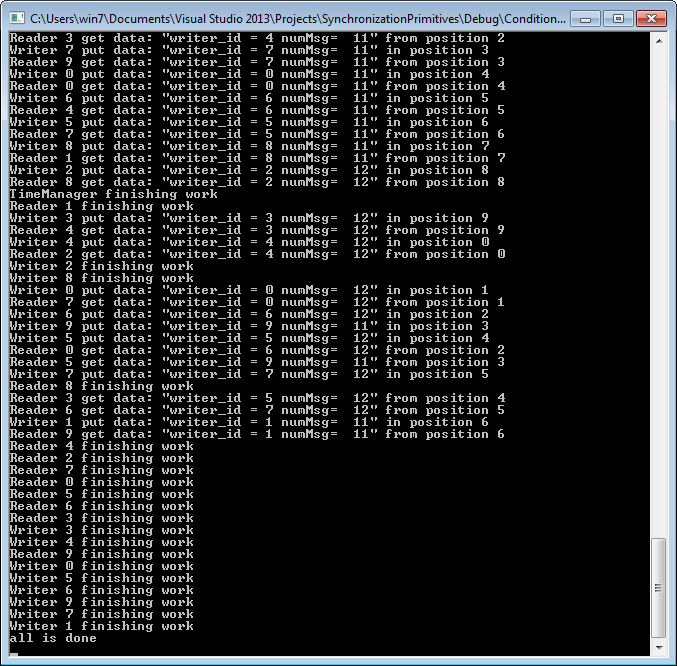
\includegraphics[scale=1]{res/005}
\caption{Условные переменные и критические секции.}
\end{figure}

\newpage
%------------------------------------------------
\subsection{Задача читатели-писатели (для потоков одного процесса)}

Рассмотрим частный случай этой задачи для демонстрации использования объектов-событий для синхронизации доступа к памяти.

Задание: необходимо решить задачу одного писателя и N читателей. Для синхронизации разрешено использовать только объекты-события, в качестве разделяемого ресурса -- разделяемую память (share memory). Писатель пишет в share memory сообщение и ждёт, пока все читатели не прочитают данное сообщение.

Задача должна быть решена сначала для потоков, принадлежащих одному процессу, а затем – разным независимым процессам.

Для этой задачи были внесены некоторые изменения в файл с сервисными функциями, которые позволили запустить только один поток-писатель. Примтивы синнхронизации (события) и общая память инициализируются в листинге 21, а используются писателем и читателями в листинге 22 и 23.

\lstinputlisting[language=C++, caption={Основной файл}]
{../../SynchronizationPrimitives/ThreadsReaderWriter/main.cpp}

\lstinputlisting[language=C++, caption={Единственный поток-писатель}]
{../../SynchronizationPrimitives/ThreadsReaderWriter/threadWriter.cpp}

\lstinputlisting[language=C++, caption={Потоки читатели}]
{../../SynchronizationPrimitives/ThreadsReaderWriter/threadReader.cpp}
\newpage

Каждый читатель, в соотвтетствии с условиями задачи, по одному разу прочитал сообщение писателя (рисунок 7).

\begin{figure}[h!]
\centering
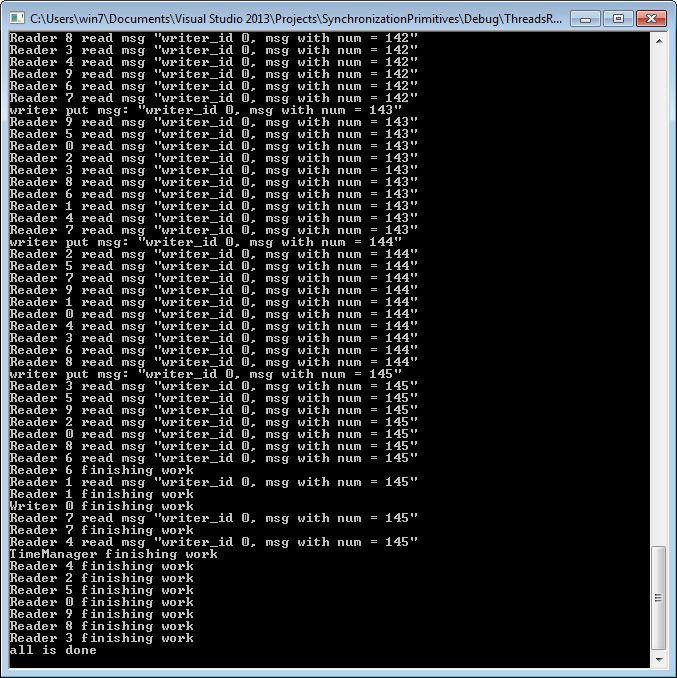
\includegraphics[scale=1]{res/006}
\caption{Задача читатели и писатели.}
\end{figure}


\newpage
%------------------------------------------------
\subsection{Задача читатели-писатели (для потоков разных процессов)}

В данной программе главный поток и поток-писатель будут принадлежать одному процессу, потоки-читатели – разным. Главный процесс создаёт процессы-читатели и 2 потока: писатель и планировщик. Для наглядности каждый процесс-читатель связан со своей консолью.

Это более сложный случай, т.к. требуется синхронизация разных процессов, а не потоков! Для этого инициализируются объекты-собтия (листинг 24) с указанием имени (по которому смогут обратиться читатели), потом стартует поток писатель (листинг 25) и запускаются (листинг 26) процессы-читатели (листинг 27).

\lstinputlisting[language=C++, caption={Основной файл}]
{../../SynchronizationPrimitives/ProcessWriter/main.cpp}

\lstinputlisting[language=C++, caption={Потоки писатели}]
{../../SynchronizationPrimitives/ProcessWriter/threadWriter.cpp}
\newpage

\lstinputlisting[language=C++, caption={Запуск кллиентских процессов}, firstline=20, lastline=76]
{../../SynchronizationPrimitives/ProcessWriter/utils.cpp}

\lstinputlisting[language=C++, caption={Потоки читатели}]
{../../SynchronizationPrimitives/ProcessReader/main.cpp}

Результат работы показан на рисунке 8, но тут интереснее взглянуть на process explorer (рисунок 9), который показывает наличие множества процессов-читателей, а среди ресурсов имена событий и общую память.

\begin{figure}[h!]
\centering
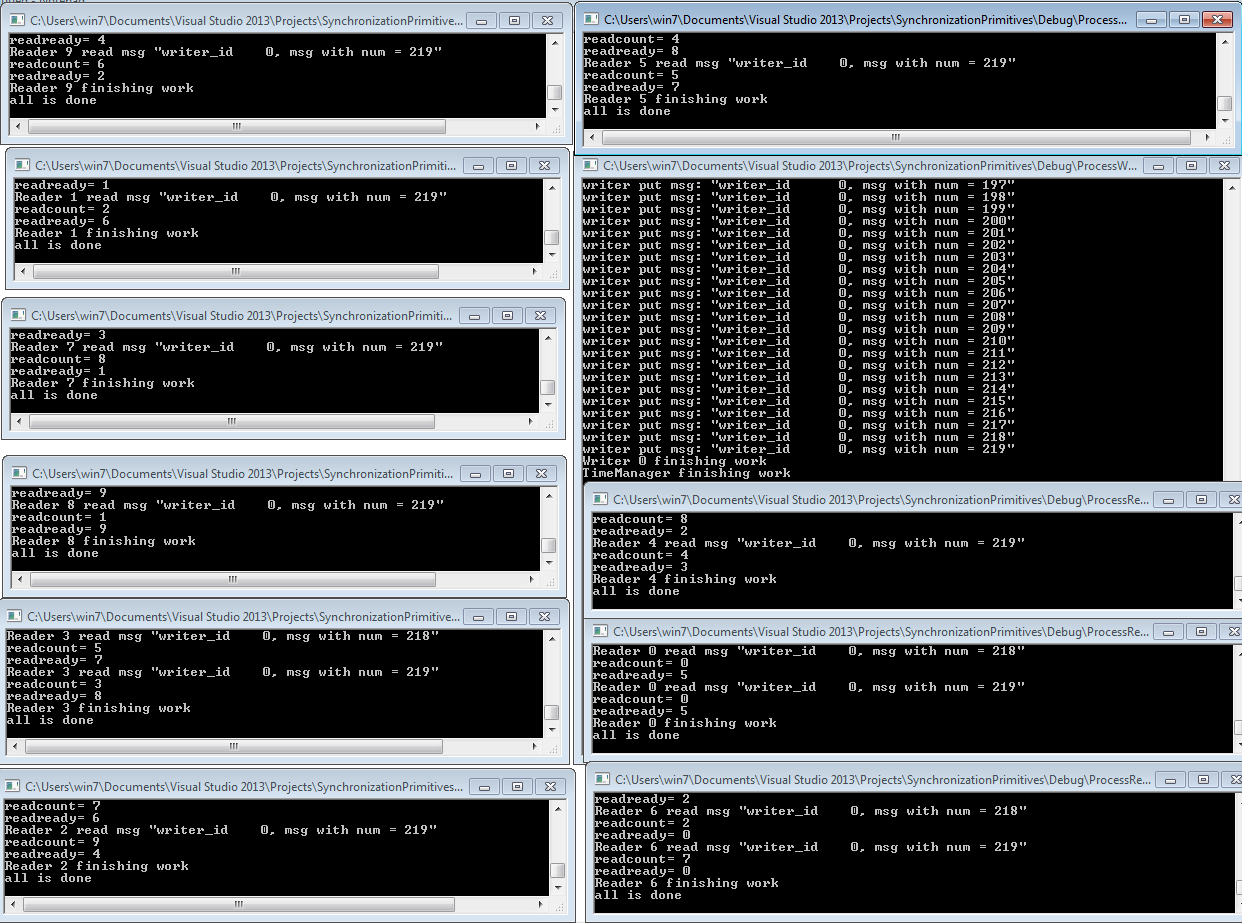
\includegraphics[scale=0.45]{res/007}
\caption{Решение задачи читатели-писатели для процессов.}
\end{figure}

\begin{figure}[h!]
\centering
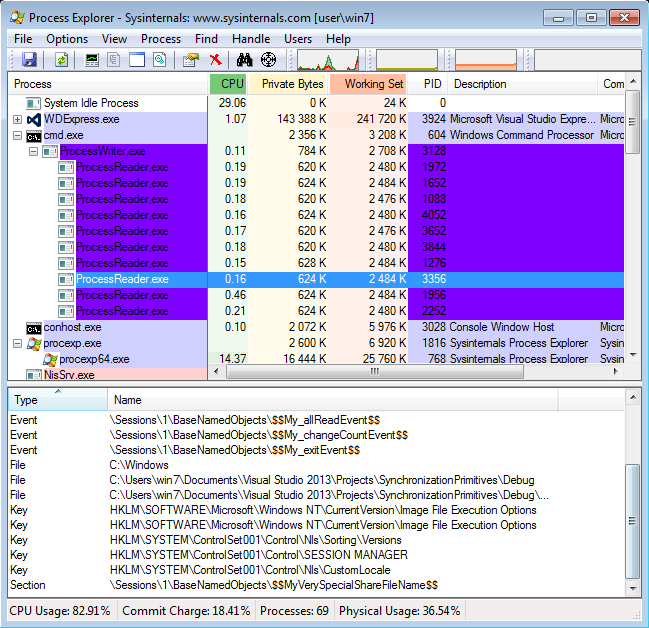
\includegraphics[scale=0.45]{res/pe_07}
\caption{Вывод process expl
orer.}
\end{figure}
\newpage

Листинг 28 содержит протокол работы единственного потока писателя, а листинг 29 - одного из читателей.

\lstinputlisting[language={},caption={Единственный писатель}]{res/ProcessWriter.ThreadWriter.log}

\lstinputlisting[language={},caption={Один из читателей}]{res/ProcessReader.1.log}

\newpage
%------------------------------------------------
\section{Модификация задачи читатели-писатели без доступа к памяти}

Требуется решить задачу читатели-писатели таким образом, чтобы читатели не имели доступа к памяти по записи. Задача сводится к тому, чтобы счётчик был под управлением какого-то одного потока (в моём случае это писатель), а остальные "отчитывались" бы ему о своей работе. Задача решена на механизме событие.

Как и в предыдушем случае, у нас есть основной файл программы (листинг 30), поток писталеь (листинг 31), сервисные функции (листинг 32) и потоки читатели (листинг 33), которые не имеют доступа на запись к общей памяти.

\lstinputlisting[language=C++, caption={Основной файл}]
{../../SynchronizationPrimitives/NoMemProcessWriter/main.cpp}

\lstinputlisting[language=C++, caption={Потоки писатели}]
{../../SynchronizationPrimitives/NoMemProcessWriter/threadWriter.cpp}

\lstinputlisting[language=C++, caption={Запуск клиентских процессов}, firstline=20, lastline=76]
{../../SynchronizationPrimitives/NoMemProcessWriter/utils.cpp}
\newpage

\lstinputlisting[language=C++, caption={Потоки читатели}]
{../../SynchronizationPrimitives/NoMemProcessReader/main.cpp}
\newpage

Результат работы на рисунке 10.

\begin{figure}[h!]
\centering
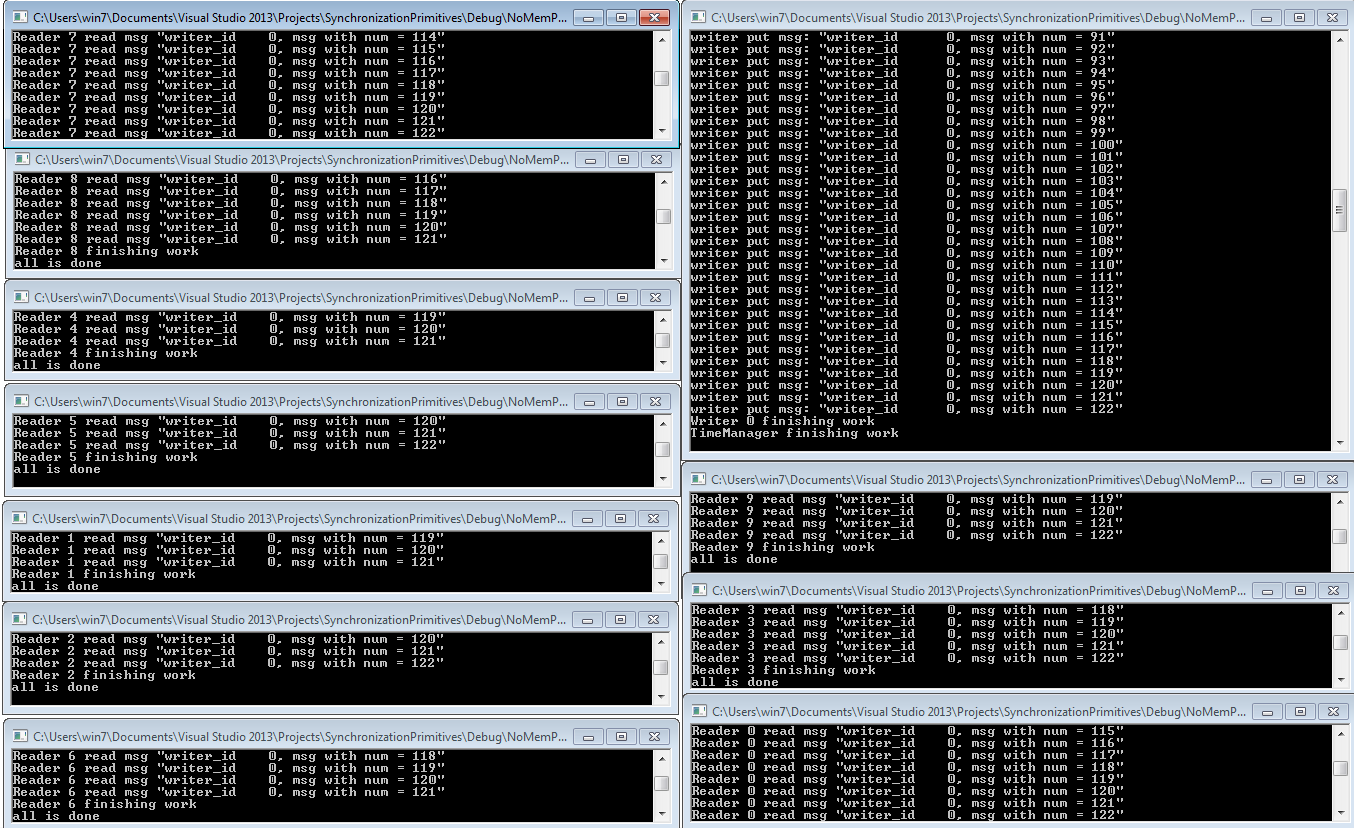
\includegraphics[scale=0.50]{res/008}
\caption{Модификация задачи читатели-писатели.}
\end{figure}

\newpage
%------------------------------------------------
\section{Рациональное решение задачи читатели-писатели}

В задаче предлагается найти более рациональное решение задачи читатели-писатели, но при имеющихся ограничениях (каждый процесс производи чтение ровно один раз) ничего существенно нового привнести невозможно, т.к. фактически всё сведётся к вырождению одних примитивов синхронизации в другие. Но предыдущую задачу, когда взаимодействие происходило в рамках одного процесса, можно рассмотреть Slim Reader/Writer (SRW) Lock, который появился в Windows Vista и позволяет накладывать различные ограничения в зависимости от задачи.
Решение с использованием Slim Reader/Writer (SRW) Lock приведено в листинге 34 (инициализация), 35 (писатели) и 36 (читатели). Сравнивать скорость этой реализации с реализациями, работающими с процессами не корректно, так что это можно рассматривать скорее как изучение ещё одного инструмента для синхронизации.

\lstinputlisting[language=C++, caption={Основной файл}]
{../../SynchronizationPrimitives/OptimalReaderWriter/main.cpp}
\newpage

\lstinputlisting[language=C++, caption={Потоки писатели}]
{../../SynchronizationPrimitives/OptimalReaderWriter/threadWriter.cpp}
\newpage

\lstinputlisting[language=C++, caption={Потоки читатели}]
{../../SynchronizationPrimitives/OptimalReaderWriter/threadReader.cpp}
\newpage

Требование по обязательному прочтению каждого сообщения каждым читателем выполняется, как видно на рисунке 11.

\begin{figure}[h!]
\centering
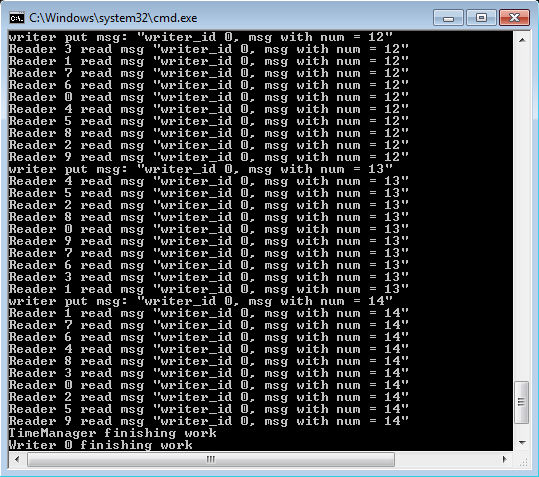
\includegraphics[scale=0.9]{res/011}
\caption{Модификация задачи читатели-писатели.}
\end{figure}

Листинг 37 показывает лог работы писталя, а листинг 38 - одного из читателей.

\lstinputlisting[language={},caption={Протокол работы писателя}]{res/OptimalReaderWriter.ThreadWriter.log}

\lstinputlisting[language={},caption={Протокол работы читателя}]{res/OptimalReaderWriter.ThreadReader.1.log}

\newpage
%------------------------------------------------
\section{Клиент-серверное приложение для полной задачи читатели-писатели}

В данной задаче появляется уже несколько писателей, а модель работы становится клиент-серверной. В качестве IPC был выбран именованный канал, а для синхронизации использованы сразу несколько инструментов: читатели ожидают на условной переменной, писатели между собой делят время при помощи критической секции, разделяемая память защищена при помощи SRW-замка.

В данной реализации (листинг 39) писатель сосредоточен в серверном модуле (всего два пистателя), а читатель (листинг 40) разнесён между серверной и клиентской частью: на сервере есть клиентский поток, который читает информацию, и отправляет её в именованный канал, где она может быть получена клиентской половиной читателя (число читателей зависит от количества запущенных клиентов и не известно заранее).

\lstinputlisting[language=C++, caption={Сервер-пистаель}]
{../../SynchronizationPrimitives/ReaderWriterServer/main.cpp}


\lstinputlisting[language=C++, caption={Клиент-читатель}]
{../../SynchronizationPrimitives/ReaderWriterClient/main.cpp}

Сервер создаёт именованный канал, и начинает писать; клиент подцепляется к каналу, и начинает читать (рисунок 12).

\begin{figure}[h!]
\centering
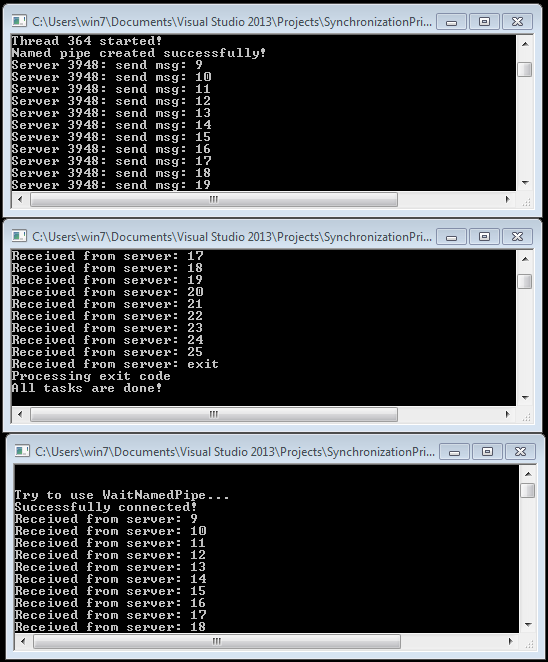
\includegraphics[scale=0.73]{res/012}
\caption{Клиент-серверное приложение}
\end{figure}

Листинг 41 показывает лог работы сервера, а листинг 42 - одного из читателей. Стоит заметить, что оба потока-писателя (3968 и 3948) пишут в свой лог в 1 файл, из-за этого в некоторых местах возникает путаница в записях. В таких случаях стоит использовать разные файлы либо использовать примитивы синхронизации для ограничения доступа к логу. Читатель тоже получает не всю информацию. Её объём завсити от времени подключения, т.е. доступ читателей к информации разграничен по времени.

\lstinputlisting[language={},caption={Протокол работы сервера с двумя писателями}]{res/ReaderWriterServer.log}

\lstinputlisting[language={},caption={Протокол работы клиента-читателя}]{res/ReaderWriterClient.292.log}


\newpage
%------------------------------------------------
\section{Сетевая версия задачи читатели-писатели}

Задача похожа на предыдущую, но взаимодействие читателей и писателей нужно осуществлять по сети. По сути, можно было взять предыдущую задачу, и использовать её в сетевом варианте (именованные каналы это позволяют), но ниже приведена реализация на сокетах. Эта реализация оказалась на много проще и гораздо лучше масштабируется.

Реализация сервера (с двумя процессами-писателями) показана в листинге 43, реализация клиента - листинг 44.

\lstinputlisting[language=C++, caption={Сервер}]
{../../SynchronizationPrimitives/NetReaderWriterServer/main.cpp}

\lstinputlisting[language=C++, caption={Клиент}]
{../../SynchronizationPrimitives/NetReaderWriterClient/main.cpp}

На рисунке 13 изображена работа приложения с двумя клиентами. На рисунке 14 показано, что работа происохдит именно через сокет.
\newpage

\begin{figure}[h!]
\centering
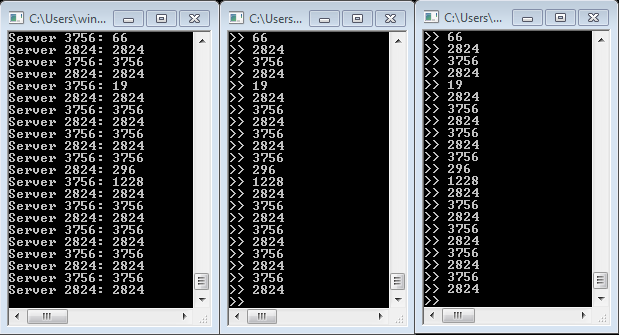
\includegraphics[scale=0.7]{res/013}
\caption{Сетевая версия задачи читатели-писатели}
\end{figure}

\begin{figure}[h!]
\centering
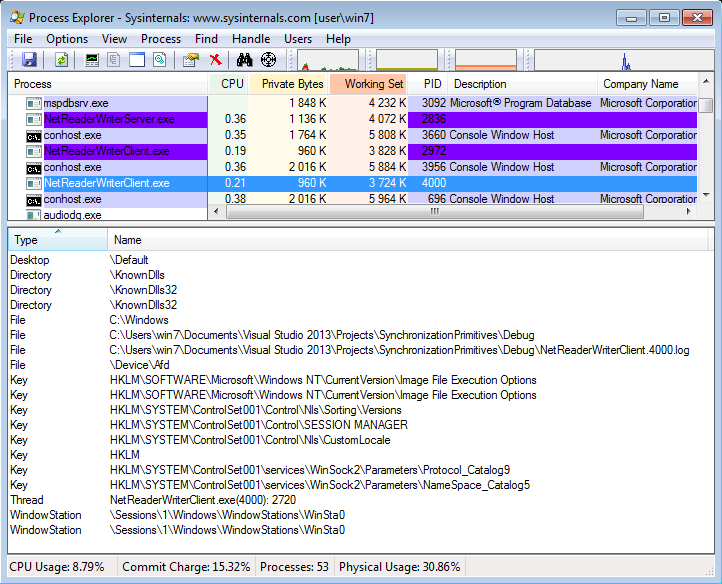
\includegraphics[scale=0.6]{res/pe_13}
\caption{Запуск process explorer для сетевой версии задачи читатели-писатели}
\end{figure}


\newpage
%------------------------------------------------
\section{Задача производители-потребители}

Отличие этой задачи в том, что теперь каждый читатель может быть писателем. Фактически, речь идёт о сетевом чате. По сути, это самая интересная задача из всех: каждый процесс тут является и производителем и потребителем, а взаимодействие происходит по сети. Обмен сообщениями устроен через список сокетов - на не больших числах (до 50 подключений) это не сказывается на работе, но при росте числа клиентов производительность начинает снижаться. Для решения этого вопроса можно добавить асинхронную рассылку уведомлений и сбалансировать нагрузку на центральном узле.

Реализация сервера представлена в листинге 45, реализация клиента - в листинге 46. При этом сложно выделить производителя и потребителя, т.к. каждый клиент является и производителем и потребителем, который должен получить каждое сообщение.

\lstinputlisting[language=C++, caption={Сервер}]
{../../SynchronizationPrimitives/FullReaderWriterServer/main.cpp}

\lstinputlisting[language=C++, caption={Клиент}]
{../../SynchronizationPrimitives/FullReaderWriterClient/main.cpp}

Рисунок 15 показывает сервер (левый верхний угол) и трёх клиентов, которые общаются между собой. Особенность реализованного протокола в том, что каждый клиент должен ввести своё имя, перед началом общения.

\begin{figure}[h!]
\centering
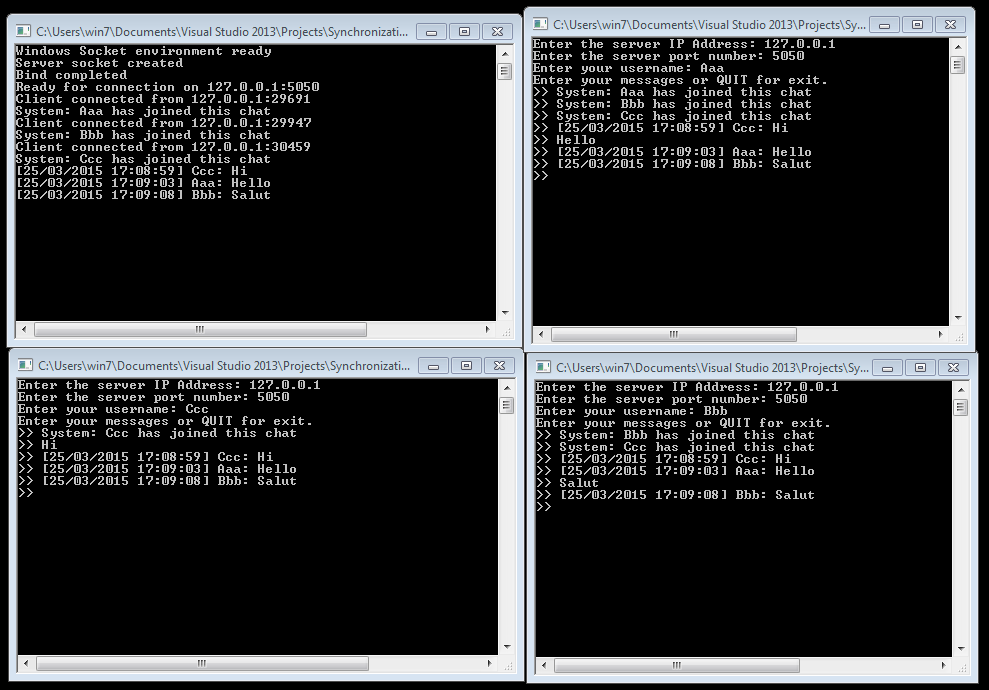
\includegraphics[scale=0.7]{res/009}
\caption{Полноценный чат на Win-сокетах.}
\end{figure}

\newpage
%------------------------------------------------
\section{Задача обедающие философы}

Классическая задача про обедающих философов. Она имеет несколько классических решений. В данном решении (листинг 47) упор сделан на то, что вовсе не обязательно вешать объект-синхронизацию на вилку, т.к. её состояние можно вывести из состояния другого философа (если он обедает, то, очевидно, вилка занята). В качестве механизма синхронизации была выбрана критическая сессия, как наиболее простая и легковесная.

\lstinputlisting[language=C++, caption={Клиент}]
{../../SynchronizationPrimitives/DiningPhilosophersProblem/main.cpp}

Результаты работы программы показаны на рисунке 16 и в листинге 48 (в этом отрывке опять набюлюдается наложение записей, т.к. несколько потоков пишут в 1 файл).

Критическая секция не является объектом ядра, так что process explorer показывает только потоки (рисунок 17).

\newpage

\begin{figure}[h!]
\centering
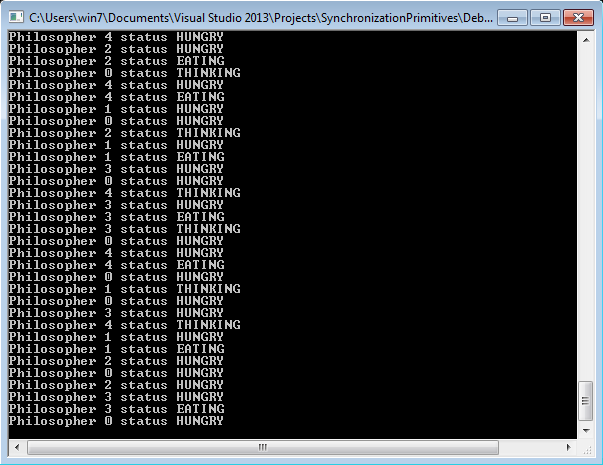
\includegraphics[scale=1]{res/010}
\caption{Эмулятор жизни философа.}
\end{figure}

\lstinputlisting[language={},caption={Отрывок протокол работы эмулятора обедающих философов}]{res/DiningPhilosophersProblem.log}


\begin{figure}[h!]
\centering
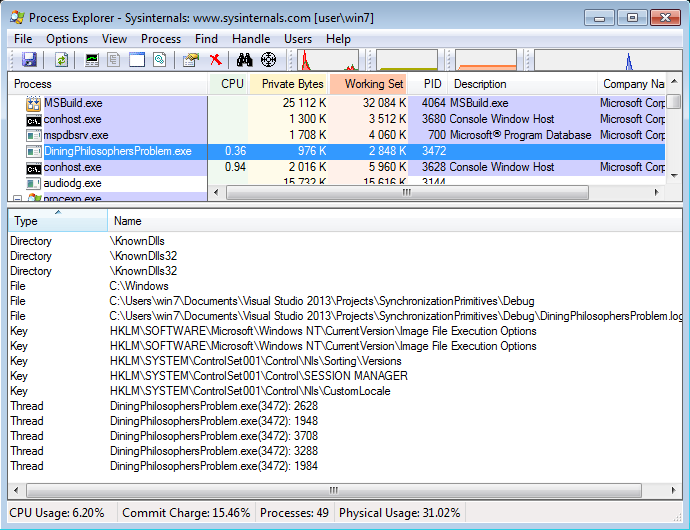
\includegraphics[scale=0.7]{res/pe_10}
\caption{вывод process explorer для задачи философов.}
\end{figure}

\newpage
%------------------------------------------------
\section*{Заключение}
\addcontentsline{toc}{section}{Заключение}

В данной работе были рассмотрены все примитивы синхронизаций, начиная с мьютексов и семафоров, и заканчивая не особо популярными - Slim Reader/Writer (SRW) Lock.

Наиболее интересной задачей была задача по полноценного производителя-потребителя. Сложность была в передаче данных от одного клиента к другому. В текущей реализации порядок доставки сообщений может быть нарушен, но это не критично, т.к. каждое сообщение имеет метку времени.

Наиболее простым механизмом является критическая секция, и именно она была использована для решения задачи философов, но, к сожалению, критическая секция может быть использована только в рамках одного процесса.

\end{document}
